\begin{tikzpicture}[node distance = 0.25\textwidth]
  \begin{scope}[yshift=0\textwidth]
    \node (raw_1) at (0, 0) {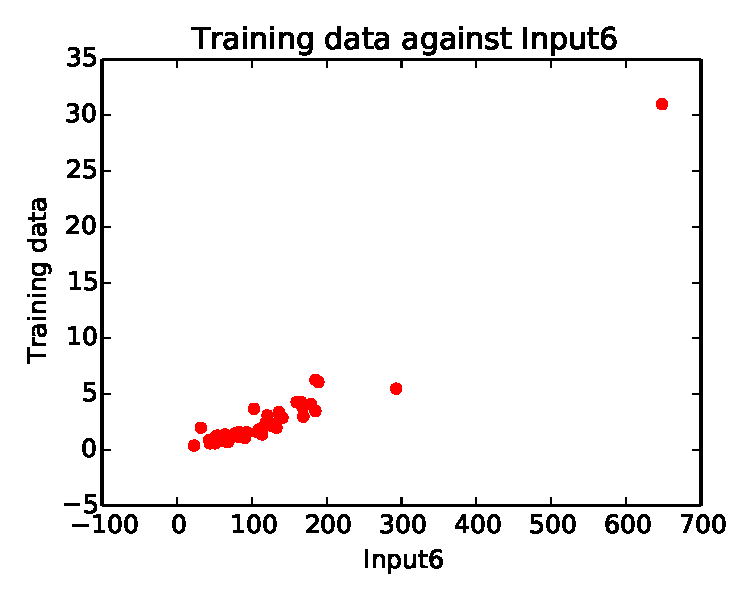
\includegraphics[width=0.25\textwidth]{../figures/auto-stat-lin-ex/lin-train-Input6.pdf}};
    \node (raw_2) [right of=raw_1] {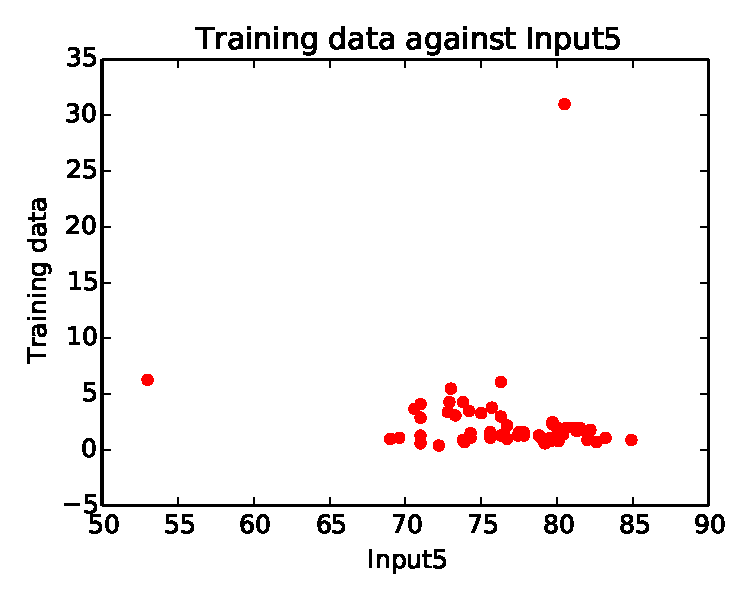
\includegraphics[width=0.25\textwidth]{../figures/auto-stat-lin-ex/lin-train-Input5.pdf}};
    \node (raw_3) [right of=raw_2] {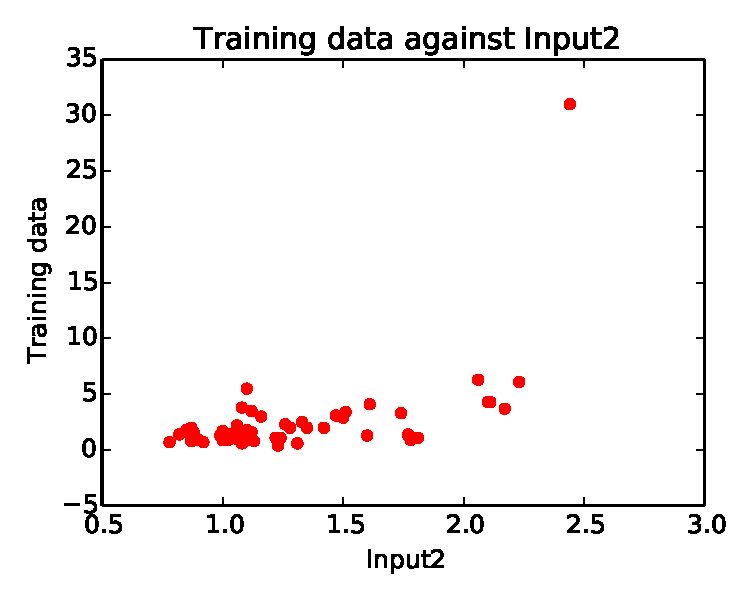
\includegraphics[width=0.25\textwidth]{../figures/auto-stat-lin-ex/lin-train-Input2.pdf}};
    \node (raw_4) [right of=raw_3] {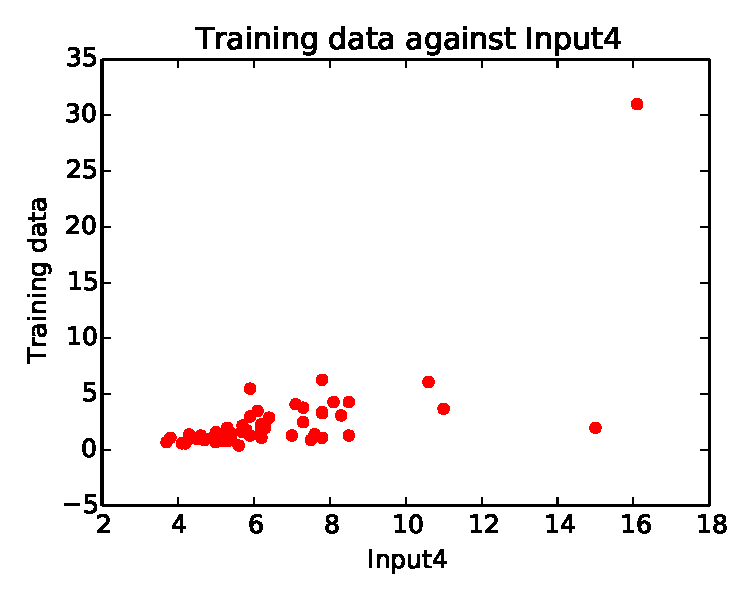
\includegraphics[width=0.25\textwidth]{../figures/auto-stat-lin-ex/lin-train-Input4.pdf}};
  \end{scope}
  \pause
  \begin{scope}[yshift=-0.25\textwidth]
    \node (raw_1) at (0, 0) {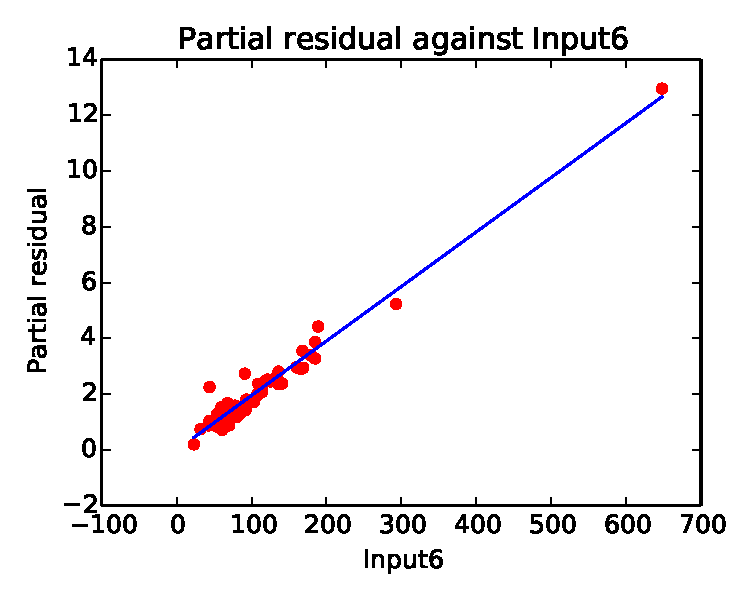
\includegraphics[width=0.25\textwidth]{../figures/auto-stat-lin-ex/lin-partial-resid-Input6.pdf}};
    \node (raw_2) [right of=raw_1] {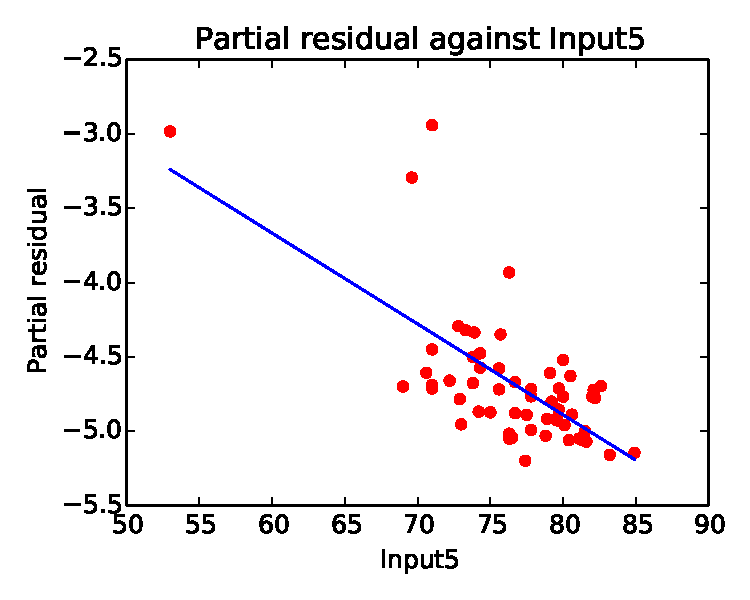
\includegraphics[width=0.25\textwidth]{../figures/auto-stat-lin-ex/lin-partial-resid-Input5.pdf}};
    \node (raw_3) [right of=raw_2] {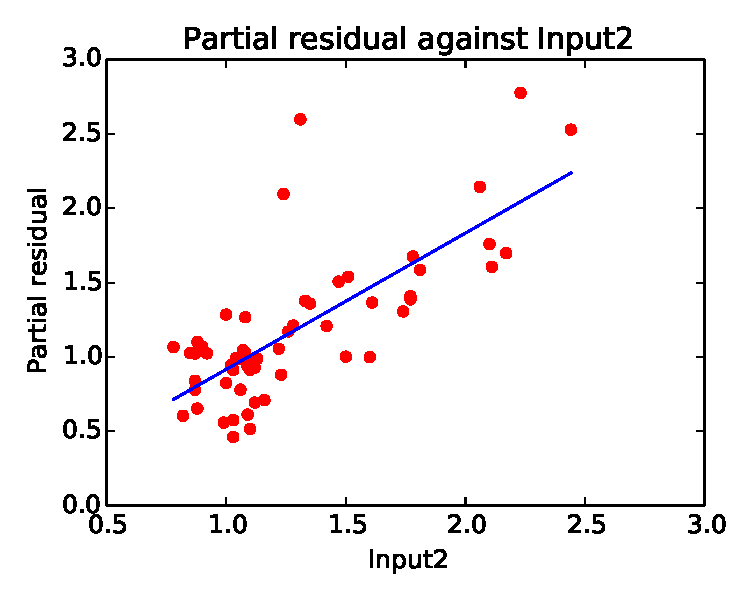
\includegraphics[width=0.25\textwidth]{../figures/auto-stat-lin-ex/lin-partial-resid-Input2.pdf}};
    \node (raw_4) [right of=raw_3] {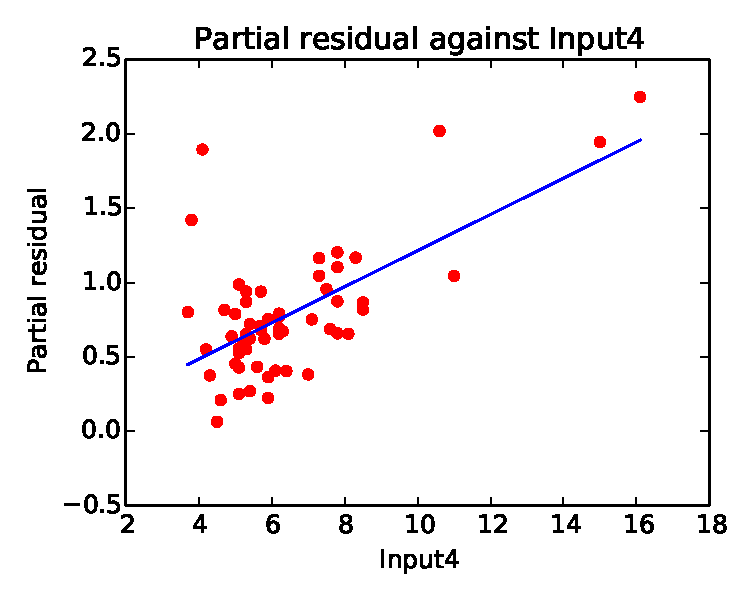
\includegraphics[width=0.25\textwidth]{../figures/auto-stat-lin-ex/lin-partial-resid-Input4.pdf}};
  \end{scope}
  \pause
  \begin{scope}[yshift=-0.45\textwidth]
    \node (quote) [text width=0.8\textwidth, align=center] at (0.4\textwidth,0)
    {``The Automatic Statistician made some sense of my data. Absolutely extraordinary.''};
  \end{scope}
\end{tikzpicture}

